\section{Sensitivity to the Review Policy}
\label{sec:sensitivity}
The calibrated threshold fixes a single operating point on the observed external benchmarks, whereas real deployments vary in both the prevalence of risky commands and the relative cost of a missed hold versus an unnecessary interruption.
\subsection{How does the class mix change the result?}
In the main template holdout, the fixed reviewer correctly approved 2,244 of the 2,320 allow-labeled commands and held 273 of the 333 hold-labeled commands. The resulting class recalls are 96.72\% and 81.98\%. Giving each class equal weight yields 89.35\% balanced accuracy. Giving each command equal weight yields 94.87\% accuracy because almost seven in eight commands were labeled allow. These summaries describe the same judgments under two sampling assumptions.

We can repeat the comparison across encoder configurations while holding the relative weight of the classes explicit. Let $\pi$ denote the assumed fraction of commands requiring review, $f$ the fraction of allow-labeled commands held, and $m$ the fraction of hold-labeled commands allowed. If the error rates within each class are fixed, the expected fraction of disagreements is
\[
  e(\pi)=(1-\pi)f+\pi m .
\]
Figure~\ref{fig:prevalence} uses the paired replay for both configurations. In that replay the full reviewer has $f=74/2320$ and $m=62/333$, and the reviewer without the general 8B model has $f=77/2320$ and $m=75/333$. At the observed prevalence of $333/2653$, the gap is 16 incorrect decisions in 2,653. At equal class weight the two error fractions are 10.90\% and 12.92\%. The larger gap under equal weighting follows from the 13 additional missed holds among 333 hold-labeled requests.

\begin{figure}[tb]
\centering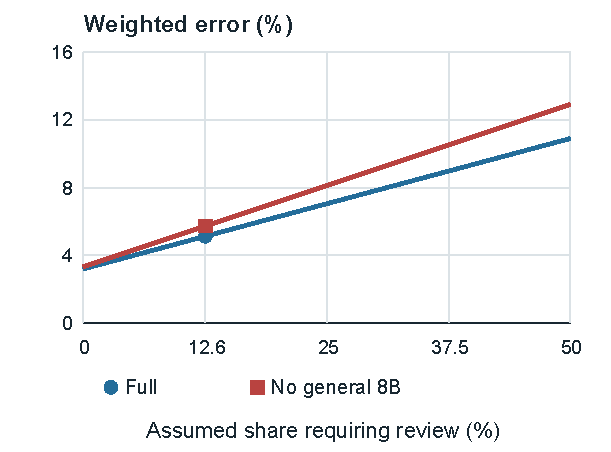
\includegraphics[width=.94\linewidth]{figures/prevalence.pdf}
\caption{Reweighting the two error rates from the matched template holdout. Markers show the observed share requiring review. Other points are calculated at hypothetical shares while keeping each class's error rate fixed. Marker and grid styling follows Yang et al.~\cite{sdcl}, Fig.~3.}
\Description{The two curves start near three percent error at zero hold prevalence. At fifty percent prevalence, the error reaches about eleven percent for the full model and thirteen percent without the general 8B.}
\label{fig:prevalence}
\end{figure}

\subsection{How much does a missed hold cost?}
The weights in $e(\pi)$ describe frequency. A separate policy choice concerns the consequences of an error. On the matched holdout, removing the joint code encoder introduced six additional false blocks and prevented three false allows. If $c_B$ is the cost of a false block and $c_A$ that of a false allow, the resulting change in total error cost is $6c_B-3c_A$. The reduced model has lower cost on these observed counts when $c_A>2c_B$, even though it has lower accuracy. Removing the general 8B increased both error counts, so its benefit in this comparison comes from shorter processing time and lower memory use. A deployment would need its own costs and class mix to value those differences.

\subsection{What can an execution harness establish?}
The opening pilot and the offline experiments observe different events. The pilot records a proposed action, the native permission decision, and a subsequent observation outside the agent. The offline experiments end when Agent Guard returns its verdict. Applying that verdict to a live action requires binding the reviewed program and relevant file state to the execution attempt. For example, a snapshot indicating that a report is still a draft describes the instant of review. If another process changes that state before execution, the earlier assessment applies to the earlier snapshot. File preservation after a denied action and completion after an allowed action are outcomes an execution harness can measure. The benchmark measures the preceding decision.
